%!TEX root = ./main.tex

The methods outlined in \textsection \ref{sec:chern_number} have proved extremely effective for characterising a wide variety of materials \cite{haldane_model_1988}, as well as providing the foundations for the modern theory of polarisation \cite{resta_macroscopic_1999}. However the definition of Chern number used also suffers from some important limitations. This is because we are forced to work in Fourier space in order to construct the Berry curvature. It is only possible to work in Fourier space when the system in question has both perfectly uniform translational symmetry, as well as living in either periodic or infinite boundary conditions. This is a serious problem since every material we encounter in the real world will fail to satisfy at least one of these conditions! Furthermore, it is not possible to apply any of these methods to quantum systems with interactions, or to systems out of equilibrium.\par
One potential solution to these problems has been the development of local Chern indicators such as the Bott Index \cite{toniolo_equivalence_2017,loring_guide_2019} and the Chern marker \cite{bianco_mapping_2011}. The idea here is to re-express the definition of Chern number in terms of a set of operators that are local, and so do not rely on the transition to Fourier space to make sense. Such a quantity should be equivalent to calculating the Chern number using $ k$-states in the case of a translationally symmetric, periodic system; however would still be possible in contexts where these conditions have been relaxed, and the notion of $k$-space breaks down. This would afford the researcher tools with which to comment on the topological characteristics of materials that had previously been out of reach using the standard methods, such as amorphous crystals \cite{agarwala_topological_2017}, quasi-periodic lattices \cite{huang_theory_2018} and systems out of equilibrium \cite{caio_topological_2019,toniolo_time-dependent_2018}. \par
In this section we start by introducing two such quantities, the Bott index and the Chern marker, giving their definitions as well as explaining how they are related. In both cases, these quantities are somewhat unstable when taken out of contexts in which the Chern number has a straightforward definition, and display a number of unexpected characteristics not explained by our definition of Chern number. 

\subsection{Bott Index}
We will work with a lattice model, where unit cells are indexed by a vector of the form $(m_x,m_y)$. The lattice has size $(L_x,L_y)$, and we have set periodic boundary conditions. Sites are indexed by 
\begin{align}
	\ket{\bf m \alpha} = \ket{\bf m} \otimes \ket{\alpha},
\end{align} 
where $\bf m$ is a vector labelling the unit cell and $\alpha$ selects a site within the unit cell. We shall use a Hamiltonian that has translational symmetry, so we may apply Bloch's theorem to obtain the form of the energy eigenstates,
\begin{align}
	\hat H &= \sum_{\bf k} \ket{\bf k}\bra{\bf k}\otimes \hat H(\bf k) \\ 
	\ket{\psi_{\bf k, n}} &= \ket{\bf k} \otimes\ket {u_{\bf k, n}},
\end{align}
where $\ket {u_{\bf k, n}}$ are the eigenstates of $\hat H(\bf k)$ and the momentum states are defined as in \textsection\ref{sec:lattice_bloch},
\begin{align}
	\ket{\bf k} = \frac{1}{\sqrt{L_x L_y}} \sum_{\bf m} e^{i \bf m \cdot \bf k} \ket {\bf m},
\end{align}
and we assume that the system has a total of $\eta$ bands, so $n \in  \{1,...,\eta\}$. Henceforth we will assume that only the $n$\ts{th} band is occupied, so we can construct a projector onto the occupied subspace, $\hat P$, and its complement, $\hat Q$.
\begin{align}
	\hat P & = \sum_{\bf k} \ket{\psi_{\bf k, n}}\bra{\psi_{\bf k, n}} \\
	\hat Q & = \sum_{\bf k,\, m \neq n} \ket{\psi_{\bf k, m}}\bra{\psi_{\bf k, m}}.
\end{align}
We also introduce a pair of operators $e^{i \delta_x \hat x}$ and $e^{i \delta_y \hat y}$, 
with
\begin{align}
\delta_x = \frac{2\pi}{L_x} ,\  \delta_y = \frac{2\pi}{L_y}.
\end{align}
In order to understand the effect of these operators, we consider their effect on the plane wave states
\begin{align}
	e^{i \delta_x \hat x}\ket{\bf k} &= \frac{1}{\sqrt{L_x L_y}} \sum_{\bf m} e^{i \delta_x \hat x} e^{i \bf m \cdot \bf k} \ket {\bf m} \\
	& = \frac{1}{\sqrt{L_x L_y}} \sum_{\bf m} e^{i \bf m \cdot (\bf k + \boldsymbol{\delta}_x)} \ket {\bf m}\\
	& = \ket{\bf k + \boldsymbol \delta_x},
\end{align}
similarly
\begin{align}
	e^{i \delta_y \hat y}\ket{\bf k} = \ket{\bf k + \boldsymbol \delta_y } 
\end{align}
Here the symbols $\boldsymbol{\delta}_x$ and $\boldsymbol{\delta}_y$ represents a vector translation in $\bf k$-space,
\begin{align}
	\boldsymbol \delta_x = \begin{pmatrix}
	\delta_x \\
	0
	\end{pmatrix}, \ \boldsymbol \delta_y = \begin{pmatrix}
	0 \\
	\delta_y
	\end{pmatrix}.
\end{align}
Thus, these operators effect a translation in $\bf k$ space by the minimum step in the reciprocal lattice. \par
Now let's look at the effect of these operators on the projector $\hat P$,
\begin{align}
	e^{i \delta_x \hat x} \hat P e^{-i \delta_x \hat x}  &=  \sum_{\bf k} e^{i \delta_x \hat x}  \ket{\bf k} \bra{\bf k} e^{-i \delta_x \hat x}\otimes \ket{u_{\bf k, n}}\bra{u_{\bf k, n}} \\
	&=  \sum_{\bf k} \ket{\bf k +\boldsymbol{\delta}_x} \bra{\bf k +\boldsymbol{\delta}_x } \otimes \ket{u_{\bf k, n}}\bra{u_{\bf k, n}} \\
	&=  \sum_{\bf k} \ket{\bf k } \bra{\bf k } \otimes \ket{u_{\bf k-\boldsymbol{\delta}_x, n}}\bra{u_{\bf k-\boldsymbol{\delta}_x , n}},
\end{align}
where the last line follows from a redefinition of $\bf k$. This is allowed as we are summing over the whole Brillouin zone. For the sake of clarity later on, we will re-express the density operator $\ket{u_{\bf k, n}}\bra{u_{\bf k, n}}$ in the following form
\begin{align}
	\ket{u_{\bf k, n}}\bra{u_{\bf k, n}} = \hat u_{\bf k, n},
\end{align}\par
so we get
\begin{align} \label{eqn:p_identity}
	e^{i \delta_x \hat x} \hat P e^{-i \delta_x \hat x}  =  \sum_{\bf k} \ket{\bf k } \bra{\bf k } \otimes \hat u_{\bf k-\boldsymbol{\delta}_x, n}.
\end{align}
Now we have enough tools to introduce the definition of the Bott index!
\begin{align}\label{eqn:bott_index}
    B(\bf A) = -\frac{N}{2\pi} \sum_\alpha \Im \bra{\bf A \alpha} \log \left [ \hat U\hat V\hat U^\dag \hat V^\dag + \hat Q \right ]\ket{ \bf A \alpha}
\end{align}
Here $N$ denotes the total number of unit cells in the system and the log is a standard matrix logarithm, defined as
\begin{align}
	\log (M) = \sum_{k=1}^\infty (-1)^{k+1} \frac{(M-\1)^k}{k}.
\end{align}
The Bott index is a local indicator, $\bf A$ is a vector that selects which unit cell in the system we are looking at, and
\begin{align}
	\hat U  = \hat P e^{i \delta_x \hat x} \hat P \\
	\hat V  = \hat P e^{i \delta_y \hat y} \hat P.
\end{align}
To make sense of this expression, let us focus on the $ \hat U\hat V\hat U^\dag \hat V^\dag$ part only, writing this out explicitly gives us
\begin{align}
	 \hat U\hat V\hat U^\dag \hat V^\dag = \hat P e^{i \delta_x \hat x} \hat P e^{i \delta_y \hat y} \hat P e^{- i \delta_x \hat x} \hat P e^{-i \delta_y \hat y} \hat P.
\end{align}
We now add in the identity in the form $e^{i \delta_x \hat x} e^{-i \delta_x \hat x} $, as well as the corresponding expression for $y$, and regroup the equation, taking advantage of the fact that $\hat x$ and $\hat y$ commute, to get
\begin{align}
	 \hat U\hat V\hat U^\dag \hat V^\dag =  \hat P
	  \left [ e^{i \delta_x \hat x} \hat P e^{-i \delta_x \hat x} \right]
	  \left [ e^{i \delta_y \hat y} e^{i \delta_x \hat x} \hat P  e^{-i \delta_y \hat y} e^{- i \delta_x \hat x } \right]
	  \left [ e^{i \delta_y \hat y} \hat P e^{-i \delta_y \hat y } \right]
	 \hat P.
\end{align}
Using eqn.~\ref{eqn:p_identity} we can now rewrite this in terms of Bloch states to get
\begin{align}
	\hat U\hat V\hat U^\dag \hat V^\dag = \sum_{\bf k} \ket{\bf k } \bra{\bf k } \otimes  \hat u_{\bf k, n}  \hat u_{\bf k -\boldsymbol{\delta}_x , n}  \hat u_{\bf k-\boldsymbol{\delta}_x-\boldsymbol{\delta}_y, n}  \hat u_{\bf k-\boldsymbol{\delta}_y, n}  \hat u_{\bf k, n}.
\end{align}
Since the first and last $\hat u$ density operator in this expression are identical, we can rewrite this in terms of a trace to get
\begin{align}
	\hat U\hat V\hat U^\dag \hat V^\dag = \sum_{\bf k} \ket{\bf k } \bra{\bf k } \otimes  \ket {u_{\bf k, n}} \bra{u_{\bf k, n}} \cdot  \tr \left [ \hat u_{\bf k, n} \hat u_{\bf k -\boldsymbol{\delta}_x , n}  \hat u_{\bf k-\boldsymbol{\delta}_x-\boldsymbol{\delta}_y, n}  \hat u_{\bf k-\boldsymbol{\delta}_y, n} \right ].
\end{align}
If we compare this to the definition of Berry flux (eqn.~\ref{eqn:berry_flux}), we see that this reduces to
\begin{align}
	\hat U\hat V\hat U^\dag \hat V^\dag = \sum_{\bf k} \ket{\bf k } \bra{\bf k } \otimes  \ket {u_{\bf k, n}} \bra{u_{\bf k, n}} \cdot r_{\bf k} e^{-i F_{\bf k-\boldsymbol{\delta}_x-\boldsymbol{\delta}_y}},
\end{align}
where $r_{\bf k}$ is just some real number that we don't care about, arising from the $u$ states not being perfectly parallel to one another. This is promising, remember we are aiming to get a sum of $F_{\bf k}$ over the whole Brillouin zone. Thus in order to extract the term in the exponential we would like to take a log. However, we cannot simply log the expression in the form we have here. This is because it only has support on the occupied subspace,
\begin{align}
    \hat U\hat V\hat U^\dag \hat V^\dag \sim \begin{pmatrix}
M &0 \\ 
 0& 0
\end{pmatrix},
\end{align}
where $M$ just indicates the presence of a nonzero operator. The presence of a null space means a log of this matrix will diverge. To remedy this, we add in the $\hat Q$ projector, 
\begin{align}
    \hat U\hat V\hat U^\dag \hat V^\dag  + \hat Q \sim \begin{pmatrix}
M &0 \\ 
 0& \1
\end{pmatrix}.
\end{align}
Now we can safely take the log of this matrix, getting the following result
\begin{align}
	\log \left [ \hat U\hat V\hat U^\dag \hat V^\dag + \hat Q \right ] = \sum_{\bf k} \ket{\bf k } \bra{\bf k } \otimes  \ket {u_{\bf k, n}} \bra{u_{\bf k, n}} \cdot \left ( \log(r_{\bf k})-i F_{\bf k-\boldsymbol{\delta}_x-\boldsymbol{\delta}_y}\right ),
\end{align}
Next we trace out the internal degree of freedom and squeeze this expression between a pair of position states $\ket {\bf A}$, selecting some arbitrary unit cell in our system. 
\begin{align}
	\sum_\alpha \bra{\bf A \alpha}\log \left [ \hat U\hat V\hat U^\dag \hat V^\dag + \hat Q \right ]   \ket{\bf A \alpha} = \sum_{\bf k} |\braket{\bf A|\bf k}|^2 \cdot  \braket{u_{\bf k, n}|u_{\bf k, n} } \cdot \left ( \log(r_{\bf k})-i F_{\bf k-\boldsymbol{\delta}_x-\boldsymbol{\delta}_y}\right ).
\end{align}
We can show that $|\braket{\bf A|\bf k}|^2 = \frac{1}{N}$ and $\braket{u_{\bf k, n}|u_{\bf k, n} } = 1$. All that is left to do is take the imaginary part, 
\begin{align}
	\sum_\alpha \Im \bra{\bf A \alpha}\log \left [ \hat U\hat V\hat U^\dag \hat V^\dag + \hat Q \right ]   \ket{\bf A \alpha} = \frac{1}{N} \sum_{\bf k} - F_{\bf k-\boldsymbol{\delta}_x-\boldsymbol{\delta}_y} .
\end{align}
Now, redefining $\bf k$ and multiplying by $-\frac{N}{2\pi}$ gives us
\begin{align}
	-\frac{N}{2\pi} \sum_\alpha \Im \bra{\bf A \alpha}\log \left [ \hat U\hat V\hat U^\dag \hat V^\dag + \hat Q \right ]   \ket{\bf A \alpha} = \frac{1}{2\pi} \sum_{\bf k}  F_{\bf k}.
\end{align}
By comparing with eqn.~\ref{eqn:discrete_chern_number}, we can see that we have arrived at an expression for the Chern number!
\begin{align}
	\mathcal Q = -\frac{N}{2\pi} \sum_\alpha \Im \bra{\bf A \alpha}\log \left [ \hat U\hat V\hat U^\dag \hat V^\dag + \hat Q \right ]   \ket{\bf A \alpha} .
\end{align}
Thus we have shown that in the case of a translationally symmetric system with periodic boundaries, the Bott index evaluated at any point in our material always exactly calculates the Chern number. Before we show some example calculations, let us introduce one more quantity.

\subsubsection{A Different Interpretation}

There is also another way to intuitively understand where the Bott index comes from, this loosely reflects the arguments presented in \cite{hastings_almost_2010}. As we saw in \textsection\ref{sec:wannier_states}, it is possible to construct a set of spatially localised states (the Wannier states) from the energy eigenstates of each band. Furthermore, these states can only be exponentially localised when we are able to define a smooth gauge across the whole of the Brillouin zone. As explained in \textsection\ref{sec:chern_smooth_gauge}, a smooth gauge is only achievable when the system has trivial Chern number. This means that the presence of a nonzero Chern number necessarily results in an obstruction to constructing a set of tightly localised Wannier states.\par
 If we were able to fully decompose the states in $\hat P$ into a set of localised states, then the $\hat x$ and $\hat y$ operators would commute when acted on the subspace spanned by $\hat P$. This would mean that the operators $\hat P e^{i \delta_x \hat x}\hat P $ and $\hat P e^{i \delta_y \hat y}\hat P $ would commute, so the Bott index would vanish. Thus the Bott index can be seen as indicating whether there is an obstruction to constructing a fully localised set of Wannier states -- telling us wether the material has nonzero Chern number.

 
 
\subsection{Chern Marker}

The Chern marker was first introduced in \cite{bianco_mapping_2011}, however we will not restate the derivation that they used. Instead we will justify the Chern marker by showing that it can be obtained from the Bott index in the limit of large system size.\par
Our starting point is the expression for Bott index, eqn.~\ref{eqn:bott_index}. We start by multiplying $\hat U$  and $\hat V$ by complex phases $e^{-i \delta_x C_x}$ and $e^{-i \delta_y C_y}$. This has no effect on the value of the Bott index, since the phases have opposite sign in $\hat U ^\dag$ and $\hat V ^\dag$.
\begin{align}
	\hat U  \rightarrow \hat P e^{i \delta_x (\hat x - C_x)} \hat P \\
	\hat V  \rightarrow \hat P e^{i \delta_y (\hat y - C_y)} \hat P.
\end{align}
As the system size becomes large, the factors $\delta_x$ and $\delta_y$ will become infinitesimally small. Around the neighbourhood of the unit cell at position $(C_x, C_y)$, the term in the exponential will be small so we can Taylor expand it,
\begin{align}
	\hat U &=  \hat P + i \delta_x \hat P \hat x_C \hat P + O(\hat x_C^2)\\
	\hat V &= \hat P + i \delta_y \hat P \hat y_C \hat P + O(\hat y_C^2)
\end{align}
where we have relabelled $ \hat x - C_x= \hat x_C$ and $ \hat y - C_y= \hat y_C$.  Using these expressions, we can re-express the operator $\hat U\hat V\hat U^\dag \hat V^\dag$ up to second order in $\delta$ as\footnote{You might have noticed that we have omitted the $\delta_x^2$ and $\delta_y^2$ terms. This is justified because those terms involve only hermitian operators, such as $ \hat P \hat x_C \hat P \hat x_C \hat P$, and these give no contribution when we take the imaginary part later.}
\begin{align}
 	\hat U\hat V\hat U^\dag \hat V^\dag = \hat P  - \delta_x \delta_y \left (  \hat P \hat x_C \hat P \hat y_C \hat P  -  \hat P \hat y_C \hat P \hat x_C \hat P \right ) + O(\delta_x^2, \delta_y^2)
\end{align}
Now we use the identities 
\begin{align}
	\hat P + \hat Q &= \1\\
	\log \left [ \1 + \delta M \right ] & \simeq M, \textup{  for  } \delta \textup{ small} 
\end{align}
to show that
\begin{align}
	\log \left [ \hat U\hat V\hat U^\dag \hat V^\dag  + Q  \right ] \simeq - \delta_x \delta_y \left [  \hat P \hat x_C \hat P, \hat P \hat y_C \hat P  \right ]
\end{align}
We can now drop the constant shifts in $\hat x_C$ and $\hat y_C$, since these vanish due to the commutator. Inserting this into the expression for Bott index, we arrive at the form of the Chern marker,
\begin{align}
 	C(\bf A)  = -2\pi i \sum_\alpha \bra{\bf A \alpha} \left [  \hat P \hat x \hat P, \hat P \hat y \hat P  \right ]  \ket{\bf A \alpha} .
\end{align}
We have skipped taking the imaginary part by noticing that the commutator is anti-Hermitian, so all of its eigenvalues are imaginary anyway, allowing us to make the substitution $\Im \rightarrow -i $.\par
This calculation comes with one important caveat. The Chern marker has an extra property that the Bott index lacks. If the system in question has finite size, then the sum of the Chern number over the whole system vanishes. This is because the sum of $C(\bf A)$ over the system is given by
\begin{align}\label{eqn:chern_sum}
	\sum_{\bf A} C(\bf A) = - 2\pi i \, \tr  \left [  \hat P \hat x \hat P, \hat P \hat y \hat P  \right ] ,
\end{align}
and the trace of a commutator is always zero in a finite Hilbert space. 

\begin{figure}[p]
\begin{center}
 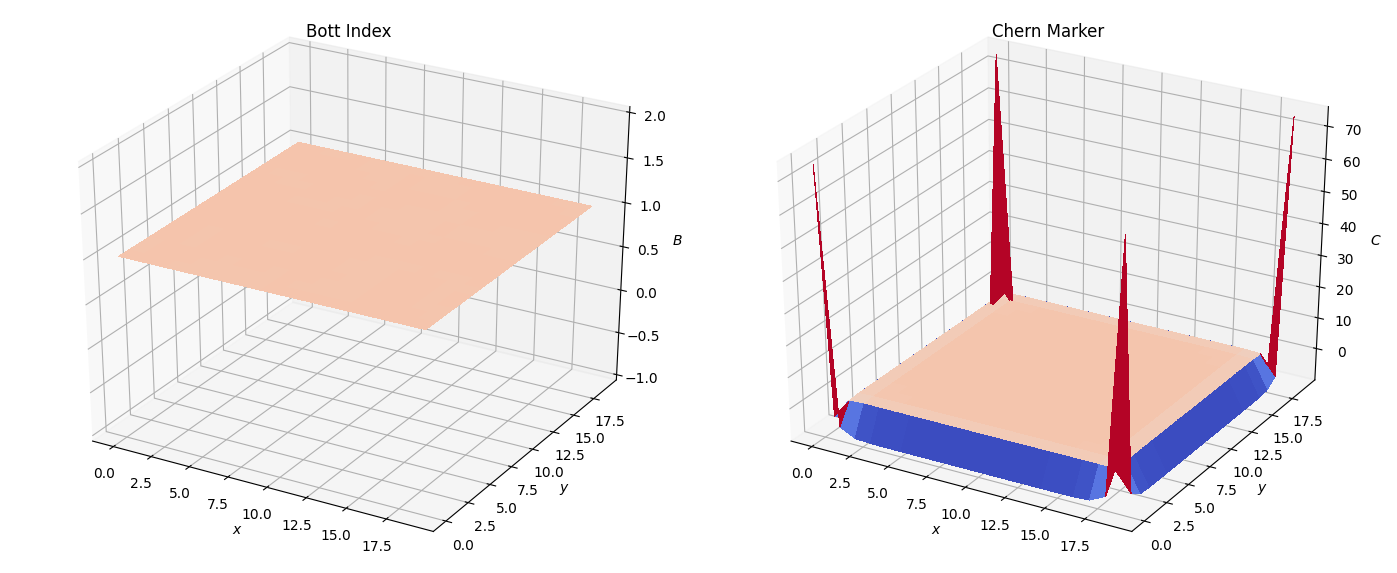
\includegraphics[width=\textwidth]{chern_bott_example}
\caption{The Bott index and Chern marker are calculated numerically for a QWZ material in periodic boundary conditions with constant $u = 1$ and $L_x = L_y = 20$.}
\label{fig:chern_bott_example}
\end{center}
\end{figure}
\begin{figure}[p]
\begin{center}
 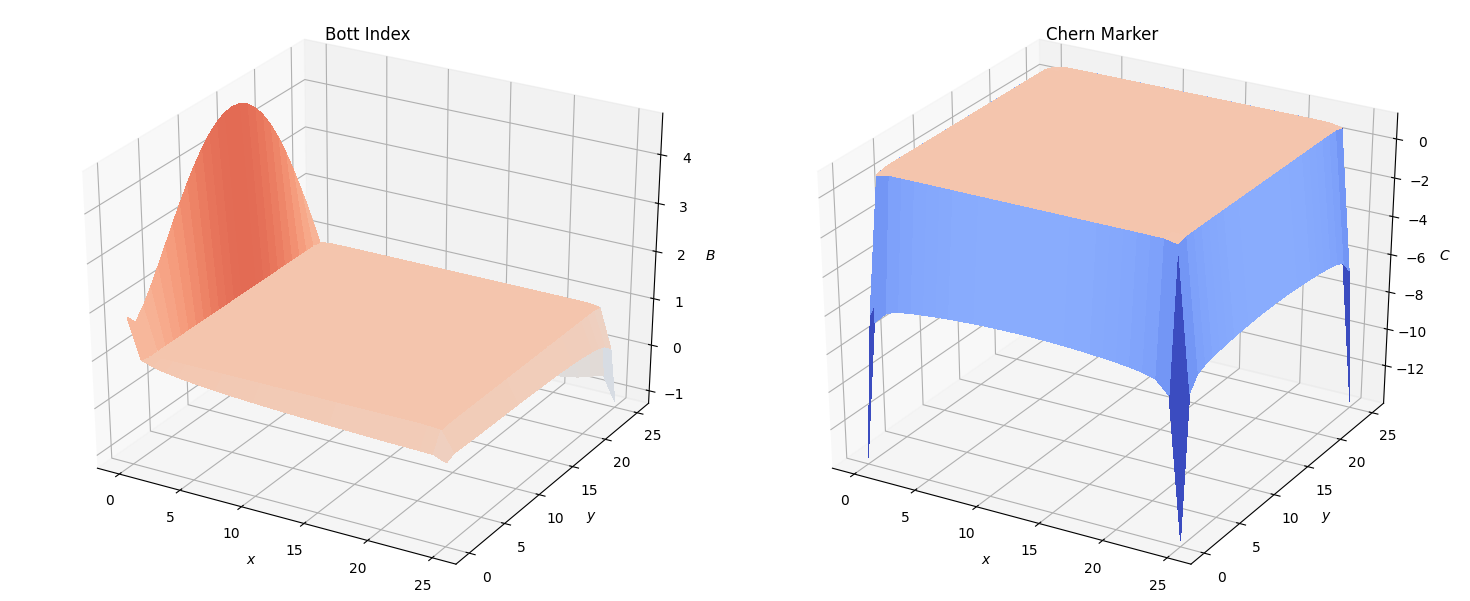
\includegraphics[width=\textwidth]{chern_bott_open}
\caption{The Bott index and Chern marker for a QWZ material with open boundaries with constant $u = 1$ and $L_x = L_y = 26$.}
\label{fig:chern_bott_open}
\end{center}
\end{figure}
\begin{figure}[p]
\begin{center}
 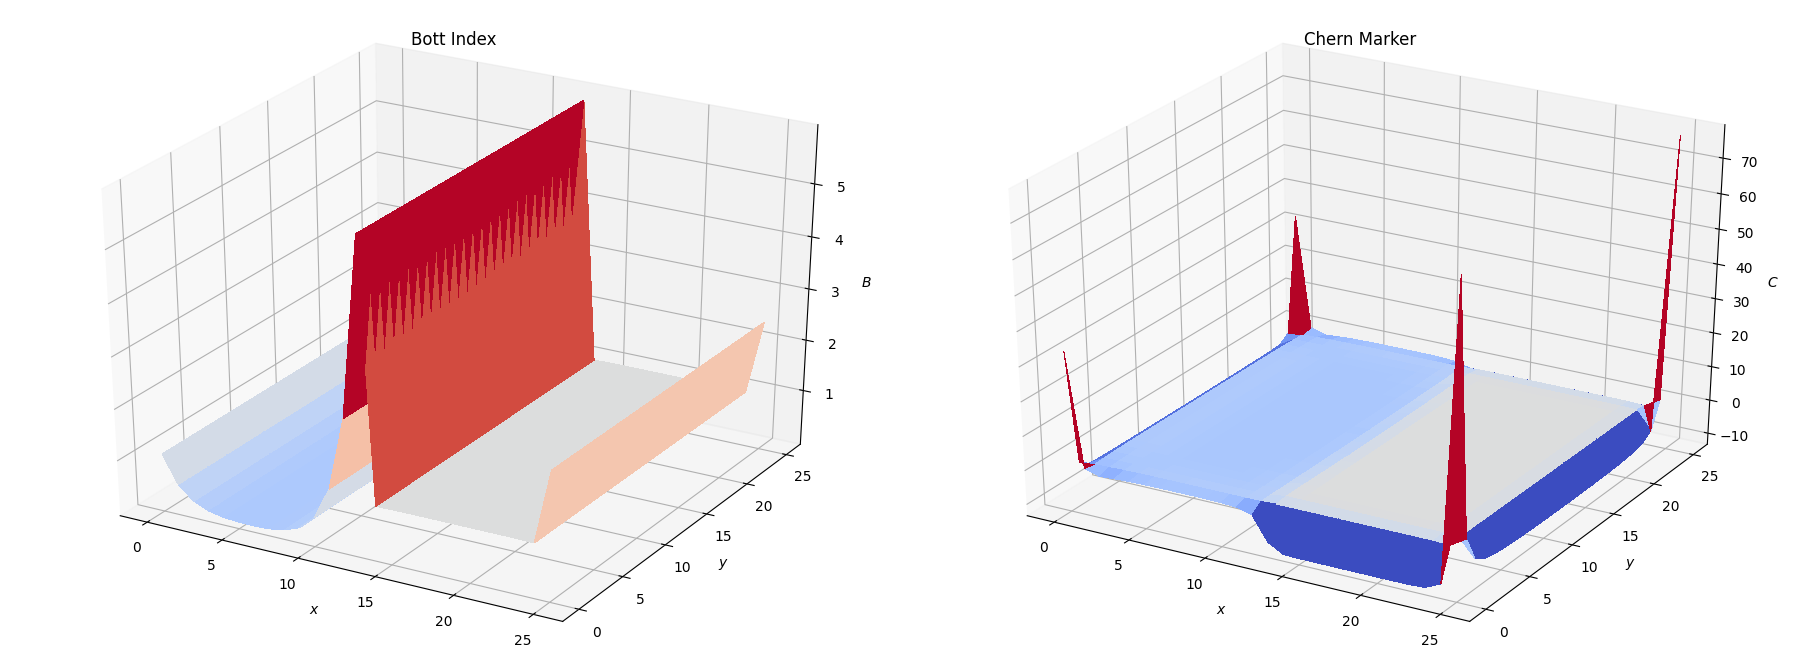
\includegraphics[width=\textwidth]{chern_bott_split_periodic}
\caption{The Bott index and Chern marker for a QWZ material with periodic boundaries with $u = 1$ for $x<13$ and $u = 2.5$ for  $x\geq13$, and $L_x = L_y = 26$. }
\label{fig:chern_bott_split_periodic}
\end{center}
\end{figure}
\begin{figure}[p]
\begin{center}
 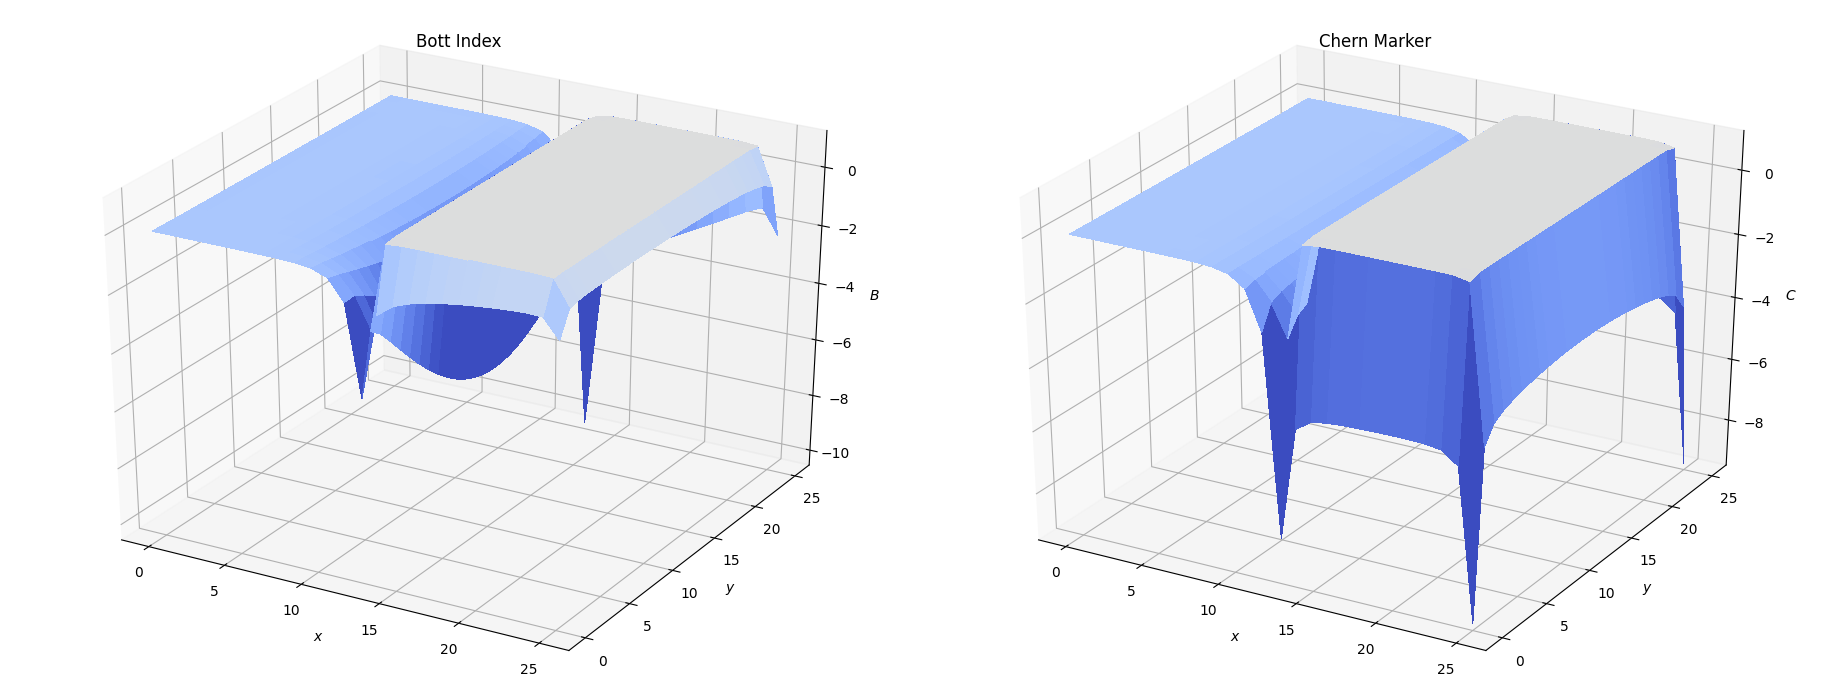
\includegraphics[width=\textwidth]{chern_bott_split_open}
\caption{The Bott index and Chern marker for a QWZ material with open boundaries with $u = 1$ for $x<13$ and $u = 2.5$ for  $x\geq13$, and $L_x = L_y = 26$. }
\label{fig:chern_bott_split_open}
\end{center}
\end{figure}
\subsection{A Gallery of Examples}

We now show a number of example calculations of the Bott index and Chern marker for a variety of different QWZ systems. We will be examining the effect that the choice of boundary conditions has on the system, as well as looking at systems with interfaces between regions of differing topological characteristic. In doing so we will be able to illustrate many of the unexpected behaviours displayed by these quantities when taken out of the setting in which they correspond exactly to the Chern number.\par
We start by looking at a uniform system with periodic boundaries, shown in fig.~\ref{fig:chern_bott_example}. Here, the Bott index exactly calculates the Chern number at every point in the system. However the Chern marker has unexpected behaviour at the edges of the system where the $\hat x$ operator jumps from $L_x-1$ to 0 (or the equivalent jump in $\hat y$). This is due to the requirement that $\sum_{\bf A} C(\bf A) = 0$, meaning that the edge behaviour must be such that it cancels out the contribution from the rest of the system. Another way of making sense of this is by seeing that the $\hat x$ operator is not well-defined in a periodic system \cite{resta_quantum-mechanical_1998}. The derivation for Chern marker is only exact when the system size becomes infinite, at which point the edge behaviour is no longer a problem since eqn.~\ref{eqn:chern_sum} is no longer a trace over a finite system.\par
Next we look at a system with open boundaries, shown in fig.~\ref{fig:chern_bott_open}. Here, the Bott index displays sharp jumps at the edges of the material. The source of this behaviour is not straightforward and will be discussed in the next section. The Chern marker also has sharp drops at the edges, ensuring that it still sums to zero. \par
Next we look at a split system with periodic boundaries, shown in fig.~\ref{fig:chern_bott_split_periodic}. Here the material has $u = 2.5$ for $x <13$ and $u = 1$ for  $x\geq13$. The Bott index evaluates the Chern number deep in the bulk of each side of the material, giving a 0 on the left and +1 on the right. However, at the interface of the two material it has sharp discontinuities. The Chern marker on the other hand has discontinuities at the edges -- due to the discontinuity in $\hat x$, but smoothly interpolates between 0 and +1 at the interface away from the edges. Finally we look at a split system with open boundaries, shown in fig.~\ref{fig:chern_bott_split_open}. Here the Bott index once again has severe discontinuities bordering the region where $Q = +1$, as does the Chern marker.\par
For the sake of brevity we have not included graphs showing the effect of varying $u$ on these local Chern indicators, however we will briefly explain it here. As $u$ moves away from 1, either towards the conducting point at $u = 0$ or at $u = 2$, the band gap narrows and the edge states permeate deeper into the bulk. This also causes the edge distortions of both the Bott index and the Chern marker to widen and thus also permeate deeper into the bulk.\par 
Throughout the rest of this document, we will focus on the Bott index. This is because the Chern marker has several features that to the author make it seem a less reliable indicator, especially as we will be primarily working with finite-size systems. The most troublesome is the condition that $C(\bf A)$ must sum to zero. This makes it difficult to draw physical interpretations from the edge-state behaviour of the Chern marker, since it forces the edge perturbations to scale with the system size. The form of the edge states is invariant to changes in the size of the system, provided that the system is already large enough that opposite edge states do not overlap significantly. This suggests that the edge behaviour of the Chern marker is not completely determined by local properties of the quantum states, as it has a global restriction. Furthermore we can see by comparing figures \ref{fig:chern_bott_split_periodic} and \ref{fig:chern_bott_split_open} that the Chern marker can change value even deep in the bulk depending on the boundary conditions, suggesting some complex global properties. The Bott index, on the other hand, only has discontinuities where edge states are present, and a better understanding of the source and shape of these discontinuities is given in \textsection\ref{sec:strip_bott}. Additionally, the Bott index better respects the symmetries of the system, being always uniform and periodic in directions where the system is uniform and periodic.\par


